\section{IPOL web interface}

current version is 3.0.

\subsection{Introduction}
The IPOL demo Web interface has been developed with HTML5, CSS3, and Jquery. 
It allows the users to execute the IPOL algorithm's with an ergonomic interface. The users can use their own data or the examples offered by each of the demos. We shall describe the modules of which the web interface is made, its flow diagram, how the asynchronous calls work, and the data types accepted.


\section{Modules}
This section will try to explain the different modules existing in the demo app. The Javascript application is made of several modules:

\begin{itemize}
	\item Inputs
	\item Upload
	\item Editor
	\item Parameters
	\item Run
	\item Results
	\item Helpers 
\end{itemize}

Each of them is described in the following sections.

\subsection{Inputs}
This module manages the blobList provided by the DDL and display them on the web page. This module is the first one loaded 
so it will make the Async calls needed to obtaing demo information using the ID from the URL, it obtains this information from 
the DemoInfo and blobs back-end modules, see figure \ref{fig:server_interaction} on page~\pageref{fig:server_interaction}. 
These two calls will obtaing the information necessary to execute the demo, allowing 
the user choose the input blobs, edit these blobs, and tweak demo execution parameters. This input module allows 
the user choose among blobs that the demo provides. These blobs are either images, videos, or audio blobs primarily. It displays 
a line of blobs or sets of blobs to choose from.


\subsection{Upload}
If the users want to use their own blobs for the demo this module lets you upload them. Every demo has predefined 
upload slots each with their own characteristics like maximum file size and maximum image size. The user is able to upload the 
minimum required number of uploads. This module listen for events in every upload slot and get the file information in order to 
upload them when the run button is pressed.


\subsection{Editor}
This module loads after the user selects a set of blobs to run the demo with or when the users upload their blobs. It loads a view of
the chosen blobs where there is a zoom and crop functions when the sets have one blob per set. When the sets have more than 
one blob per set, the user will have the possibility to compare them with the corresponding 'Compare button', but not a crop 
an area.

\subsection{Parameters}
This module renders the parameters of the demo described in the DDL after the user chooses blobs to use with the demo. 
Parameters have as many types DDL specifies, so the interface renders each type accordingly.

\subsection{Run}
This module will send all the blobs and requirements needed to run the demo on the servers and will send this information to 
the core module. The answer will be either a success message with enough information to render the results or an error message 
that will show an aproximation of what failed during execution.

\subsection{Results}
This module will print the results the demorunner returns letting the user compare the input and results.

\subsection{Helpers}
This module act as an interface for common utility methods like read and write to sessionStorage, make HTTP requests and 
read the origin of the chosen blobs for the demo, this could be blobset, meaning blobs are chosen from the ones offered by the 
demo, and upload, meaning the user has uploaded his own blobs.

\begin{figure}[h]
	\centering
	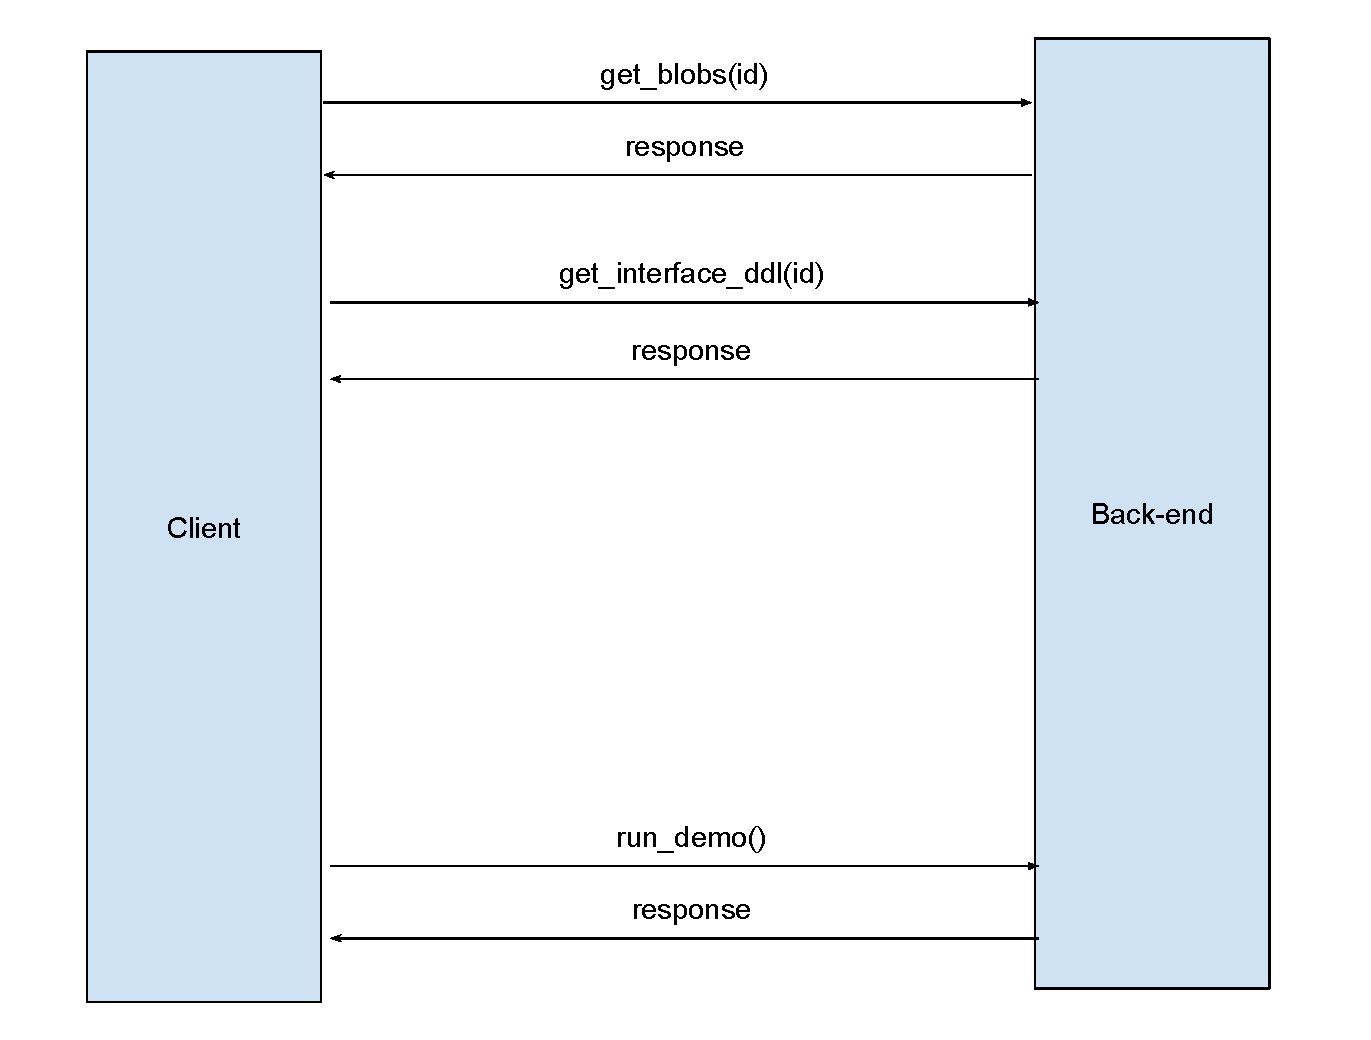
\includegraphics[width=\textwidth]{images/client_server_interaction}
	\caption{Client-server interation} 
	\label{fig:server_interaction}
\end{figure}

%--------------------------------------------------------------------------------

\section{Flow diagram}
When the application is loaded, the input module will locate the demo according to its ID. This ID is a get parameter from the URL.
Once the demo has this ID parameter, the main file, demo.js will load the different html files into the DOM. They have been divided 
into several files to improve mantainability and coupling.

After this process is done, the app will continue rendering the main section to the DOM, containing in this case the blobs viewer and 
the blob upload dialog. The information regarding the DDL and the blobs specification will be saved in sessionStorage once it 
has been retrieved by the async calls for easy access.

\begin{figure}[h]
	\centering
	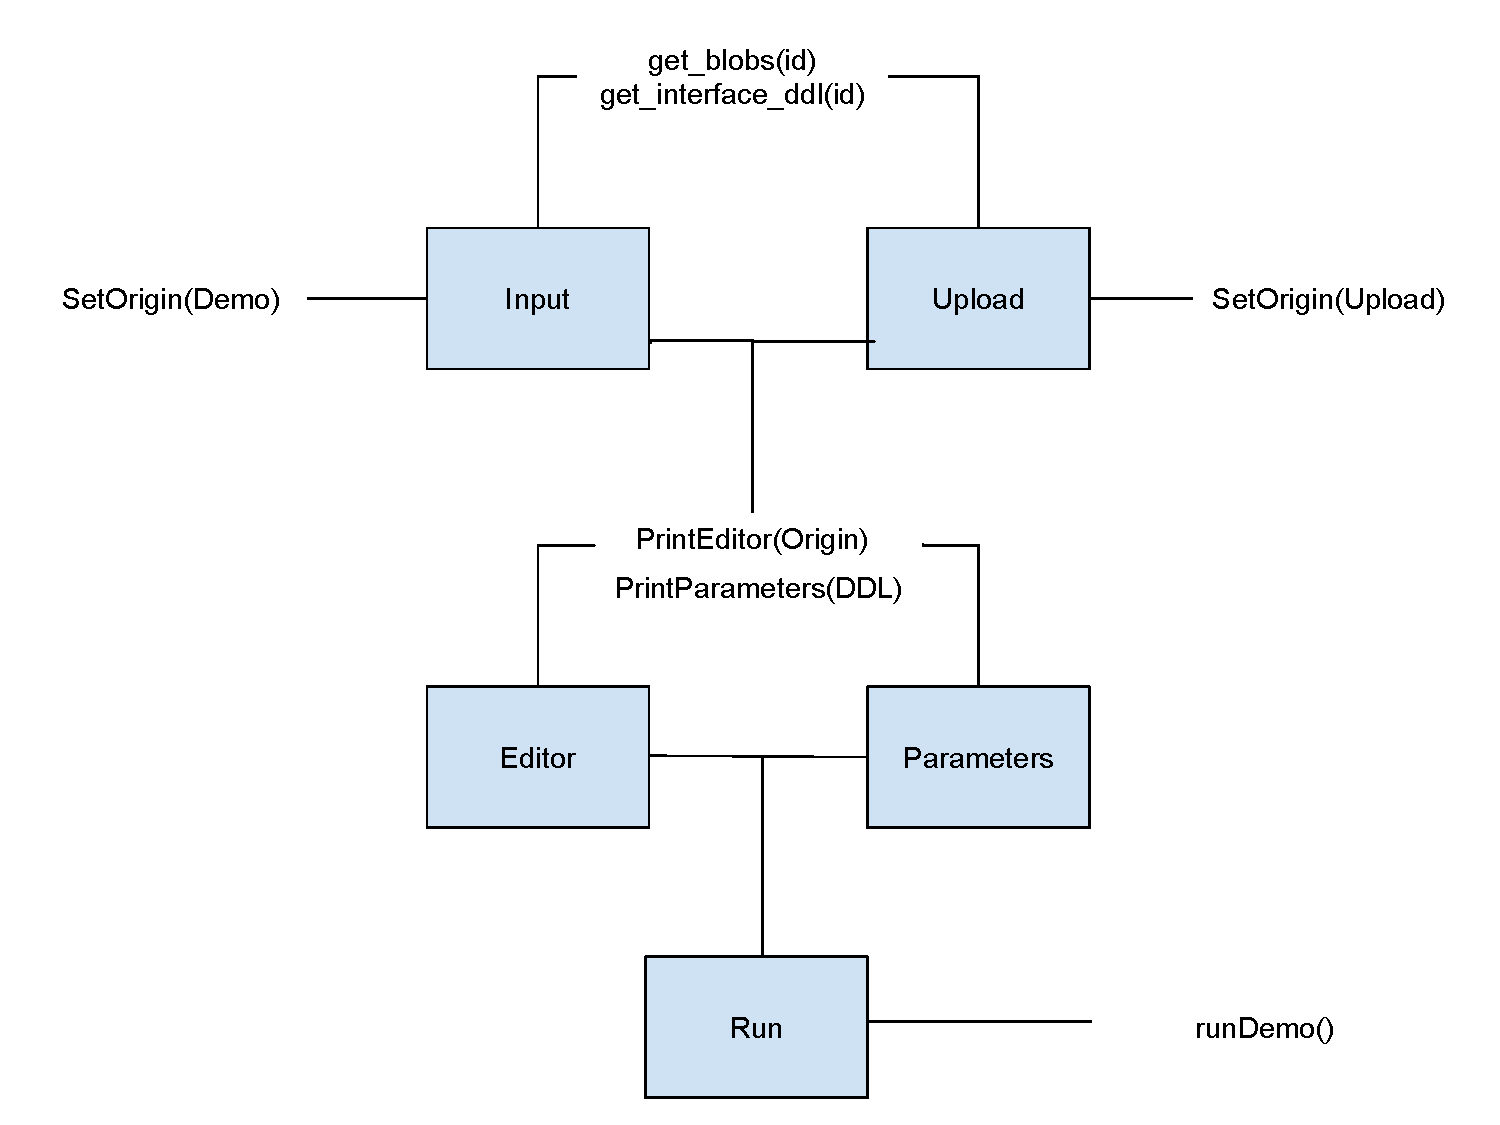
\includegraphics[width=\textwidth]{images/flow}
	\caption{Flow diagram} 
	\label{fig:flow_diagram}
\end{figure} 


As shown in figure  \ref{fig:flow_diagram}, either input or upload modules will pass 
information to the following modules. Each will set a variable in sessionStorage that will indicate if the user has chosen to 
upload blobs for the demo or a default blob from the list. If this variable is not set, it means the demo has no inputs defined 
in the DDL.

After the user chooses a blob, the editor and parameter modules will load independently and wait for changes. The Editor control 
will allow to either zoom, crop, and compare blobs if it is possible, as well as do inpainting operations when the demo requires it. 
The parameters will be modifiable according to the DDL specification values and will be stored in a variable in order to achieve 
parameter visibility dependence and to send this data when the run button is pressed.

After the user hits the run button an http post will be executed to run the demo and send the necessary information and wait for 
a response. When the response is obtained it will either print the results interface or the error message.

%--------------------------------------------------------------------------------

\subsection{External modules}

The IPOL demo Web interface uses external libraries for extra functionalities.
Currently it uses:

\begin{itemize}
\item Cropper.js: Cropper.js it is a simple image cropping JQuery plugin. It is used in the editor panel with the image blobs.
\end{itemize}

%--------------------------------------------------------------------------------

\subsection{Async calls}
The IPOL demo Web interface uses Async calls to get the necessary information from the IPOL server.

The current version uses Async calls for:
\begin{itemize}
\item Get the demo ddl: Used to show the inputs description and the upload modal in the Inputs panel, also uses this information to show the parameters.
\item Get blobs: Used to show the blobs in the inputs panel.
\item Run demo: It will send all parameters needed to run the demo and will responde with either the results of the demo or an error response.
\end{itemize}

%--------------------------------------------------------------------------------

\subsection{Data types}
The IPOL platform supports images, audio and video files to use in demos. The new web interface 
allows to choose a set with any combination of images, audio and video. Depending on the data types and sets length options will vary. 
If a set contains multiple images, the user will be able to compare and make zoom using any image on the set. If the user chooses a set with only 
one image blob, options will depend on DDL limitations and will include zoom and crop features, as well as inprinting editing.
